The non-linear model is simulated using a square wave and a chirp input
covering the entire operating range in terms of amplitude, assuming $\delta v =
0$. The simulation results are compared with experimental data using the
same input data in Fig.-\ref{fig::sq_valid} and Fig.-\ref{fig::chirp_valid}.
These figures indicate that the model parameters are estimated with reasonable
accuracy. Any discrepancies between the simulation and experimental data can
primarily be attributed to non-zero $\delta v$ and sensor noise.
%===
\begin{multicols}{2}
 \begin{figure}[H]
    \centering
    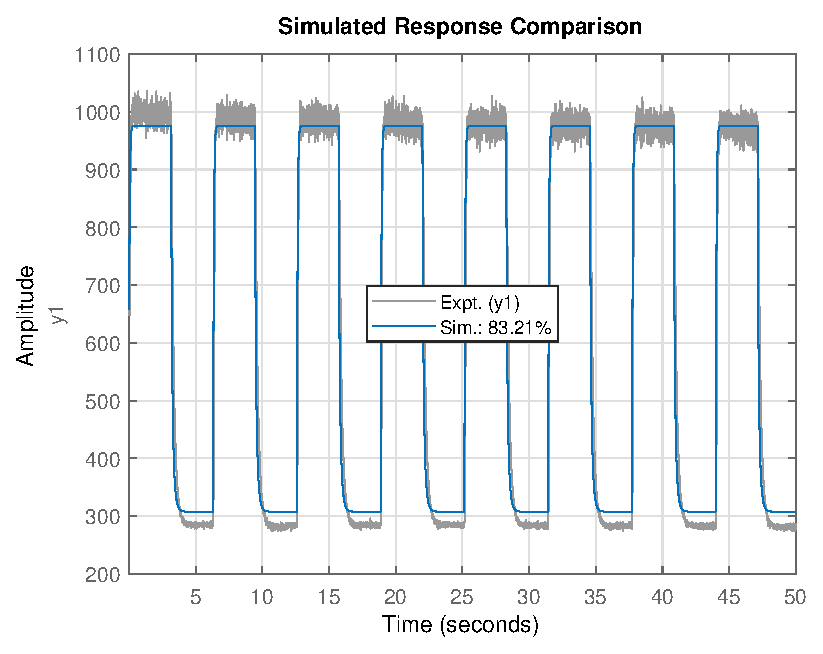
\includegraphics[width = 0.49\textwidth]{Part2/figs/3_figs/nl_valid/square_validation.eps}
    \caption{Square Wave Input Response}
    \label{fig::sq_valid}
\end{figure}
\begin{figure}[H]
    \centering
    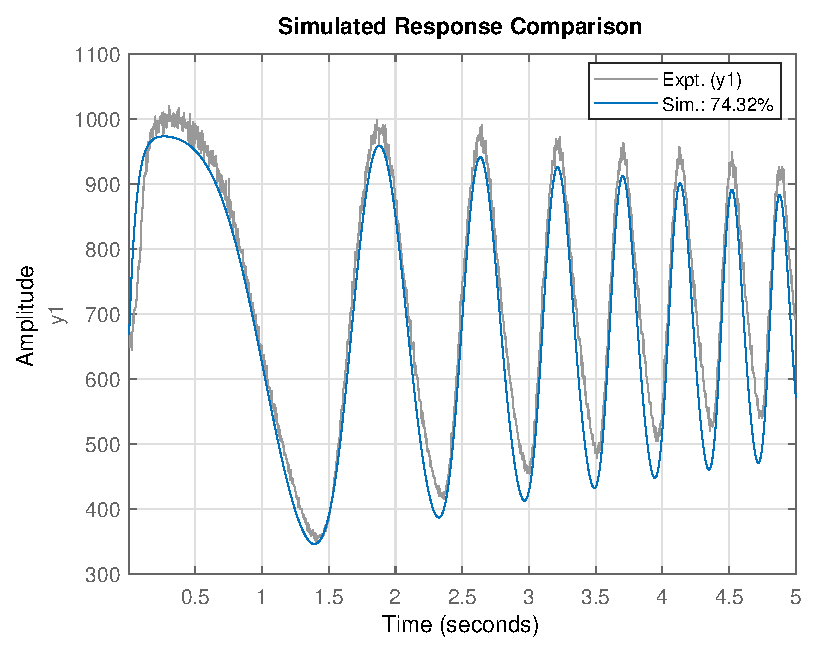
\includegraphics[width = 0.49\textwidth]{Part2/figs/3_figs/nl_valid/chirp_validation.eps}
    \caption{Chirp Input Response}
    \label{fig::chirp_valid}
\end{figure}
\end{multicols}
